\chapter{Introduction}

% tl;dr --- to be filled out \today.

% stuff is awesome -- biology and its new data

Since the first sequencing and assembly of the human genome~\cite{FirstHumanGenome}, this confluence of chemistry, general and molecular biology, genetics, and medicine bore a new field of computational biology --- and it continues to grow and present new challenges which stem from the number and complexity of the hypotheses it generates and sheer volumes of data to be analyzed simultaneously. Sequencing technologies have vastly improved since then resulting in a sharp descrease in costs which, in turn, helped sequencing machines become a commonplace in many research centers, forensic labs, and hospitals. Advances in DNA sequencing coincided with a rapid development of other high-throughput techniques that captured interactions between proteins~\cite{yeast2hybrid,TAPMS}, dependencies between metabolites, genes, and gene products~\cite{ChipSeq,GeneKnockouts}, rates of gene transcription~\cite{RNAseq} and protein translation~\cite{riboseq} offering rich data to investigate the inner workings of the cells. In turn, newly available data called for novel computational techniques that would help scientists to extract meaningful insights from these large multidimensional observations.

% complex data #1 -- PPI

One such high-throughput technique used gene expression as an indicator of the physical interactions between proteins: a yeast transcription factor GAL4 was separated into two parts with each part bearing one of the essential pieces, the binding and the activating domains. The GAL4 domains have to be directly interacting or be in close proximity to activate expression of the downstream gene~\cite{XXX}. When the two GAL4 fragments are fused with two different proteins, and those proteins --- called \textit{bait} and \textit{prey} --- can physically interact, the GAL4 fragments can come close together and form a functional transcription factor, causing the downstream gene to express~\cite{XXX}. This technique can be scaled up to screen for interactions over hundreds of protein pairs~\cite{Ito 2001}, and the pairwise protein interactions can be summarized into a single protein-protein interaction (PPI) network where nodes represent the individual proteins and edges connect pairs of proteins that allowed GAL4 domains to come close to each other to activate the gene (XXX which gene). This network will have some interesting properties: when compared to random networks, PPIs (XXX: on eppi, which one) are more connected (although very sparse), have longer average shortest paths, and its degree distribution is highly skewed with few high degree nodes and a long tail of nodes of degree 1 or 2~\cite{Zhu et al 2007}. Such networks also tend to have local subsets of nodes that share many edges to other nodes within the subset, but have few connections to the rest of the network --- such groups of proteins may actually form protein complexes, be co-located in the cell, and are likely to perform a similar function~\cite{ProteinComplexesPPI}.

% XXX other methods - tap-ms, GCNs.

% % clustering PPI -- gives us functional annotations. clustering gives ambiguous results

However, identifying such groups of proteins is a non-trivial task. Computationally, the problem of finding a decomposition of a network into disjoint groups of nodes that maximize some objective is hard~\cite{ModularityNPhard}, even if the network is sparse and scale-free~\cite{XXX}. Circumventing the problem's computational hardness, scientists developed many heuristic approaches to cluster PPIs and biological networks in general~\cite{ReviewBiologicalNetworksclustering}. XXX discuss approach 1. XXX discuss approach 2. Strikingly, protein sets recovered by one algorithm differ in size, number, and composition from protein sets suggested by other algorithms~\cite{blah}. To futher complicate the matters, it has been shown that even a single algorithm may produce different, equally good results: a study by Navlakha et al~\cite{SaketModularity} modified the popular modularity~\cite{Modularity} clustering algorithm to force it to generate all optimal and near-optimal solutions on a small network of social interactions in a karate club, and showed that XXX. Q: How should scientists decide which predicted protein complexes are real?

In fact, neither of these clusterings is wrong and neither of them offers a comprehensive analysis of the network. Each clustering algorithm and its results offer a unique summary of the data from a different perspective. When comparing results of nine (XXX) different algorithms for PPI complexes in \textit{Arabidopsis thaliana}, we observe that a large core component of the network (XXX nodes) is recovered by all nine algorithms, even though individual results suggested that the core must appear alongside many other proteins (see Chapter~\ref{chapter:coral}). To allow systematic analysis of multiple alternative clustering results, we developed an analysis and visualization tool Coral that guides users from entry-level overview statistics to in-depth comparisons of co-clustering behavior for individual proteins under different clustering regimes. We discuss metrics for comparing such clustering results and present a workflow that allows to systematically investigate proposed complexes. To aid in selection of the groups of proteins that are consistently placed in the same clsuter, we present an approach that finds the most consistently clustered groups of nodes and demonstrate the effectiveness and the need for such an approach by analyzing the protein-protein interaction network of a model organism \textit{A. thaliana}.

% alternative solutions, most robust subsets -- domains

% XXX most robust subsets, + alternative solutions = domains

The algorithm for identifying the most reliable protein complexes found another unexpected application when modeling the three-dimensional folding of the human nuclear DNA. Our view of the human genome is often skewed towards its commonly used linear representation: as an $x$ coordinate in genome browsers~\cite{GenomeBrowser}, as a backbone for genome assembly methods~\cite{RandomGenomeAssemblyMethod}, or in genome comparison tools~\cite{DotPlot}. This assumption of linearity is justified when used in these methods, however, the eukaryote genome is neatly packed in a non-random fashion and its position is mostly restricted to a specific parts of the nucleus during the interphase stage, the stage when most of the active gene expression and regulation happens in the lifecycle of a cell~\cite{GenomeOrganizationReview}. 
3C captures this genomic organization.
Data is an aggregation over millions of cells.
Identifying the most robust substructures -- can use the algo from coral above.
Like Navlakha study, not the only optimal decomposition of the genome. Can modify it to sample optima and nearoptimal solutions; when analyzed together, we can say with a measure of confidence that genomes display a strong hierarchy with smaller domains being fully contained in larger domains. See chapter~\ref{chapter:domains}.

% Protein interactions obtained through the tandem affinity purification (TAP) method capture whole protein complexes; when TAP step is coupled with mass spectrometry (MS), researchers can discern the individual proteins comprising the complex. Like GCNs, PPI networks contain on the order of thousands of nodes and tens to hundreds of edges~\cite{citeAThalsMain,someEcoliOrYeast}. The progress towards the full proteome of a species: about a decade later after the publication of the TAP-MS protocol, about one third of proteins for a model organism \textit{Arabidopsis thaliana} remained uncharacterized~\cite{cite62}. PPI networks generated through these high throughput methods were then used to assign function to novel proteins. the introduction Multiple algorithms for clustering the network are available~\cite{} that find highly connected subsets of proteins; with downstream methods aiming at inferring function, cellular localization, or the biological process the novel proteins are part of. 

% complex data #2 -- GCNs

% These new data provided a first glimpse into how organisms operate on a molecular level on a global scale --- the scale of thousands of genes and proteins at a time, along with their complex interactions and dependencies. For example, microarray panels~\cite{microarray} and, later, RNA-seq~\cite{RNAseq} experiments measure gene expression for large numbers of genes simultaneously; these measurements serve as a snapshot of the system under specific conditions at a particular time. The measurements taken under different conditions --- e.g. prior and after administering a drug to a cell culture --- can be compared to each other and point to genes for which the expression levels change significantly between the two conditions. Such \textit{co-expressed} genes may belong to the same drug response pathway and we can start building a co-expression network where nodes are the genes in question and edges connect genes that display a co-expression relationship. These co-expression relationships can be further refined as we repeat the experiment and observe the same cell culture under other conditions. We now can mine the resulting gene co-expression network (GCN) for groups of genes that were consistently co-expressed --- such genes are putatively controlled by the same cellular mechanism and may perform the same function in the cell. We can further use these strongly related groups of genes to annotate those genes for which the function is not yet known by considering the functional annotations of its neighbors.




% global view vs local view -- sometimes need to consider the local view more, ego networks

Analysis of complex data, such as protein interaction or gene co-expression networks~\cite{GSNs}, gives us a global perspective on the cooperation within cells on molecular level, however, to understand the workings of a single protein complex or a specific metabolic pathway, we would want to consider the network at a local level and observe it over time or under various conditions. 
XXX give an example of drug absorption, then go on to describe contributions. 
We developed a visualization approach that focuses on local neighborhoods around a single node and tracks topological changes over time. We use a dynamic social network of jazz musicians that captures their interactions over the course of a hundred years, however, the same design principles will easily carry over to a dynamic biological network. The principles used in that visualization --- interactivity, exploration, details-on-demand --- follow HCI principles and apply to dynamic biological networks in equal measure.

% large volumes of data

As the name suggests, high-throughput experiments generate large volumes of  data. Coupled with the need to repeat experiments multiple times under different conditions, over time, or across large cohorts of patients, as well as the need to maintain technical replicates to control experimental noise, it is easy to see how the rates of data generation quickly make data storage a central problem (XXX cornerstone?). Data compression has long been a topic of active research~\cite{CompressionReview} going back to 1940s when Shannon derived a limit on lossless compression~\cite{Shannon} and Huffman introduced frequency-based optimal Huffman codes~\cite{Huffman}. Data compression techniques allow to store data in less space, enable easier data exchange, and even allow for error correction should part of the data become corrupt~\cite{smth}. However, traditional compression techniques, like Lempel-Zip~\cite{LempelZiv}, were developed for text or image~\cite{GIF} compression and are unable to exploit the structure present in biological data. For example, sorting the short DNA sequences before compressing it with Lempel-Ziv can improve compression ratio by up to an order of magnitude, however, Lempel-Ziv algorithm assumes that the order in which characters appear can not be altered and thus can not take advantage of this simple improvement. 

XXX discuss some of the specialized compression techniques for biological data. Despite these advances in compression of biological data, both traditional and specialized compression algorithms~\cite{BAM,CRAM,Quip,SCALCE} require that data is fully decompressed before researcher can run any analyses. That means that every analysis has to account for additional time to decompress and then compress te data again and has to allocate additional space for the decompressed data. XXX how we address these problems. Later in this thesis, we investigate compression methods for one of the most abundant data types in computational biology --- the nucleotide sequences.



%%%%%%%%%%%%%%%%%%%%%%%%%%%%%%%%%%%%%%%%%%%%%%%%%%%%%%%%%%%%%%%%%%%%%%%%%%%%%%%
%%
%%
%%
%%%%%%%%%%%%%%%%%%%%%%%%%%%%%%%%%%%%%%%%%%%%%%%%%%%%%%%%%%%%%%%%%%%%%%%%%%%%%%%
\section{Major contributions}

We outline the problems addressed in this thesis and the specific contributions made while researching these topics:

\begin{itemize}
  \item \textbf{Visualization and inference of stable subsets in ensembles of classifications}

  We develop new and adapt existing visualizations useful for evaluation and comparison of collections of annotations derived from large datasets through various classification and clustering strategies. We integrate these visualizations into a single comprehensive application that allows to perform a variety of analyses on these classification results. We develop algorithms that reorder data in a way that exposes patterns and helps to identify prominent substructures more easily. Our novel algorithm for core finding automatically extracts annotations that are most consistent across all sets of assigned labels. We use our tool to perform a detailed analysis of clusters of protein-protein interactions in \textit{A. thaliana} plant and identify robust cluster cores that are significantly enriched for Gene Ontology~\cite{GeneOntology} terms and can be used in downstream analyses with greater confidence than clusters generated by a single algorithm.

  % \item \textbf{Augmented search in Sequence Read Archive (SRA)}
  % SHARQ

  \item \textbf{Visual exploration of large dynamic networks}

  We propose an egocentric network view as the main visualization to use when  studying large graphs that change over time. We augment the view by developing node and edge glyphs that summarize the interactions taking place before and after the current point in time. We develop a node ordering algorithm that minimizes node occlusion and improves graph readability over the lifetime of the egonetwork. We implement our ideas in a web application centered around a graph of interactions between jazz musicians spanning a hundred years.

  \item \textbf{Identification of topological domains in the ensembles of chromatin contacts}

  % From coral - Armatus XXX
  We extend the algorithm for identifying robust subsets of annotations from our earlier work to the problem of finding densely packed areas of chromatin (\textit{topological domains}). Our algorithm is faster, requires less parameters, and generates domains that are significantly different from domains identified by existing methods, however, are biologically significant and are more enriched for the chromatin markers associated with gene regulation. Our algorithm scales well with the increasing data resolution providing an opportunity to study genome folding and organisation in cell in fine detail. Additionally, we are able to capture domains at different length scales that allows us to evaluate, for the first time, the hierarchical structure of the chromatin.

  \item \textbf{Compression methods for sequencing and alignment data}

  % Huffmer, Referee XXX
  We propose novel ways to compress sequencing data using information shared across several related datasets and develop new algorithms for rapid compression of sequence alignments. We achieve up to 8 times better compression rates than other state of the art tools on the sequencing data, provide significant savings in space for other data types, and outperform state of the art tools on all but one dataset overall. We propose a novel infrastructure where related alignment data are separated into disjoint streams allowing for better compression of data within the stream. These separable data streams allow us to download and use data streams independently of each other furhter reducing download sizes. Our modular organisation of data allows us to perform computations on compressed data directly without fully reconstructing the original alignments thus speeding up common sequence analyses by orders of magnitude.

\end{itemize}

%  both numerical analyses and vis are important

This underlines the need for visualization when working with data. A single solution may be persuasive unless you see/or somehow else familiarize yourself w/ the whole space of solutions. Visualization relies on human intutition to help see that. numerical analysis alone may be misleading. visualization can speed up hypothesis generation and testing -- citation? to insight faster than considering some of the standard metrics. in this thesis, we consider visualization as a means to observe network dynamics over time and to analyse alternative solutions -- areas where coming up with a hypothesis is a complex task.

%%
%% Anscombe's quartet 
%%
\begin{figure}[ht]
  \centering
  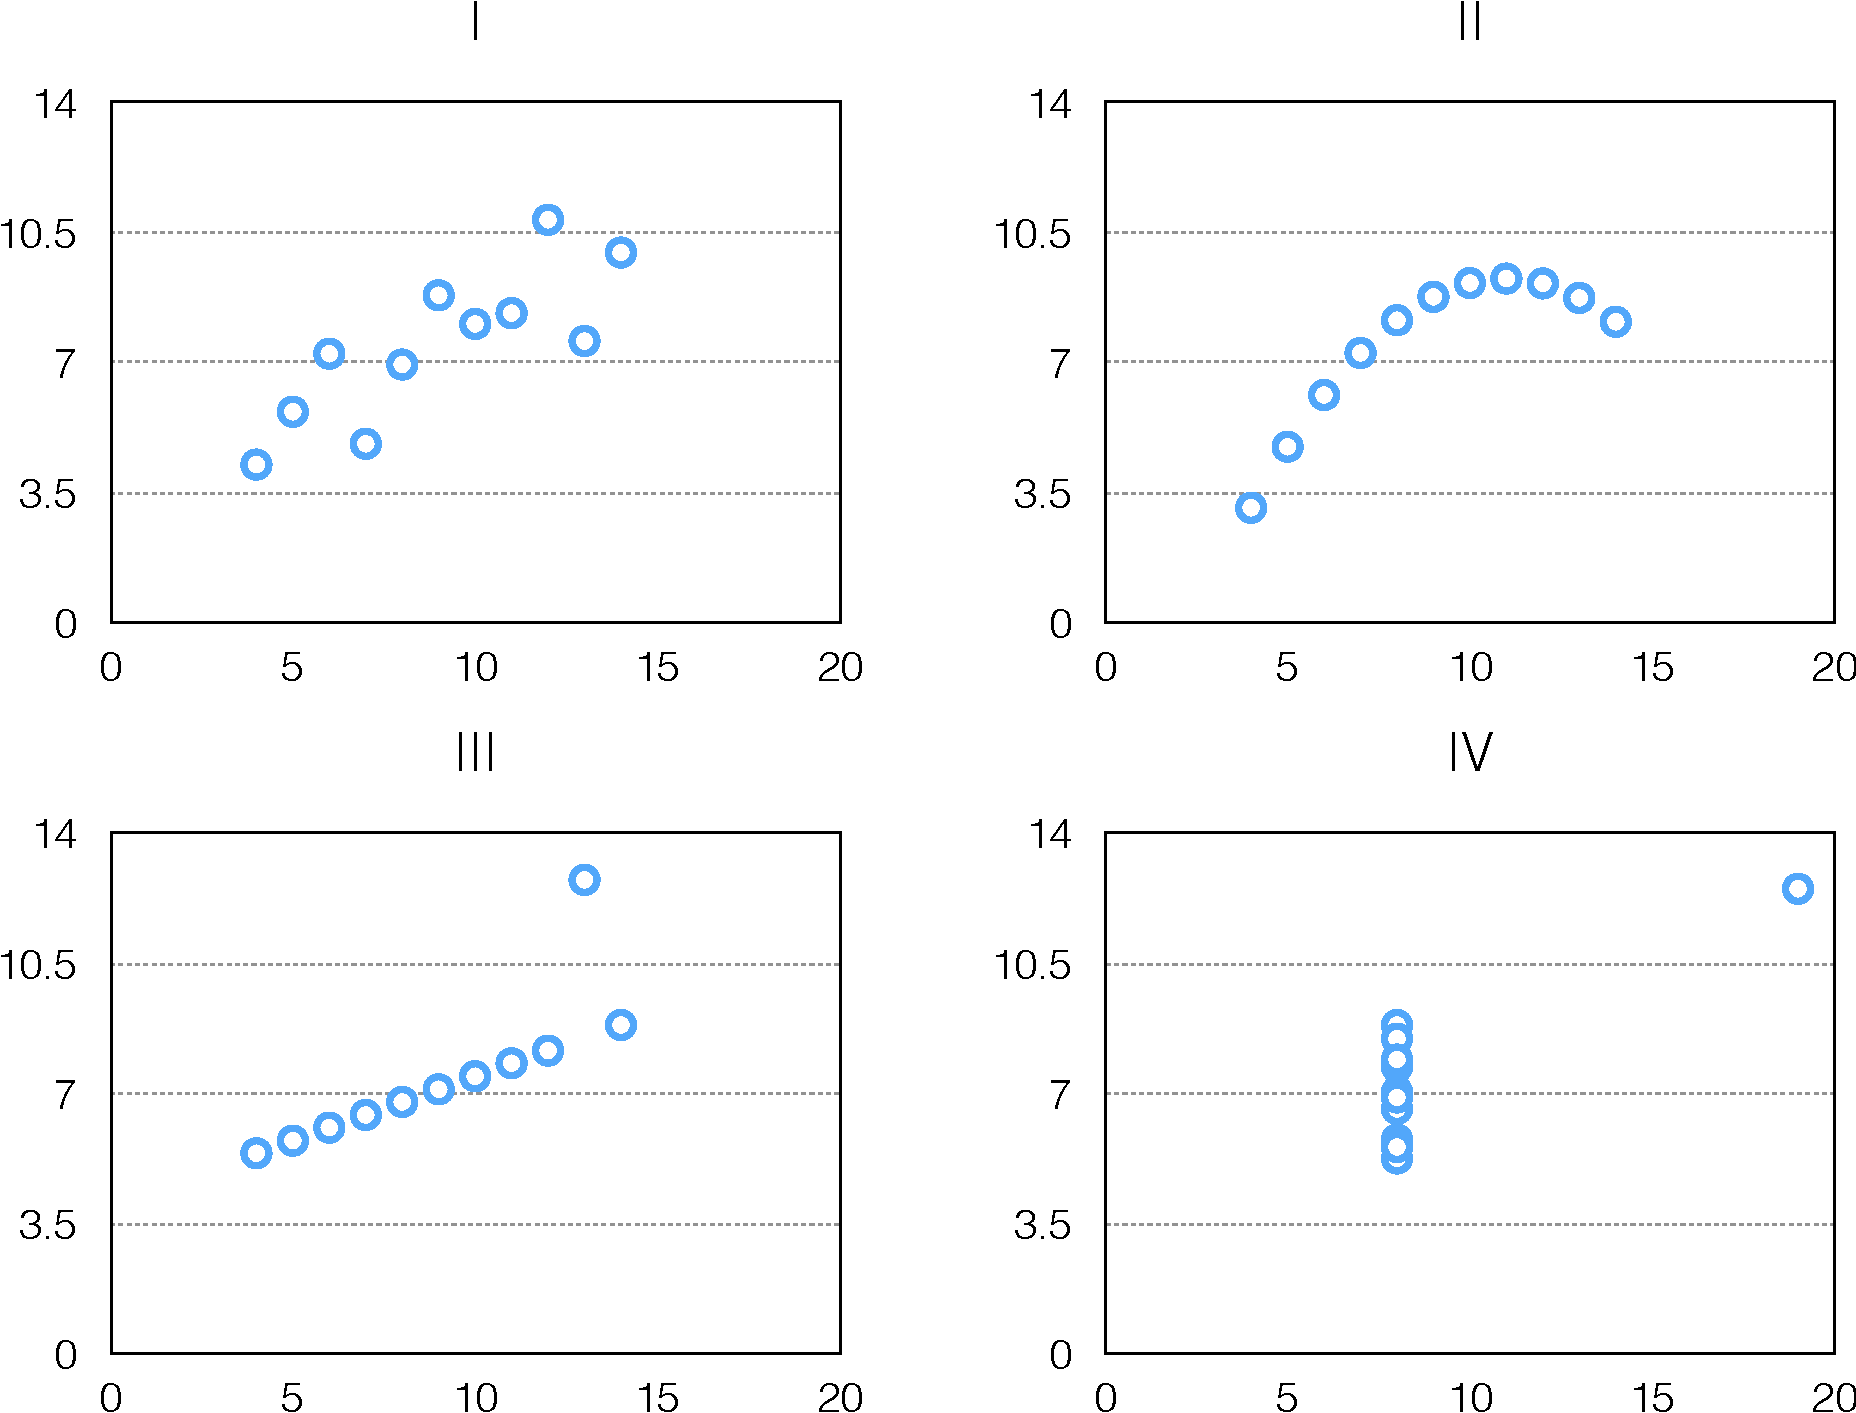
\includegraphics[width=0.8\linewidth]{figures/anscombes_quartet}
  \caption{\textbf{Anscombe's quartet.} Statistician F. Anscombe constructed these four data series to stress the importance of plotting the data before computing its summary statistics. These four sets of data points are indistinguishable when considering their $x$ and $y$ mean, variance, correlation, and linear regression, yet are strikingly different when visualized.}
  \label{fig:intro:anscombe}
\end{figure}


Visualization is an important first step when working with a new set of data as it provides the means to assess the overall shape of the data, its distribution, and to detect outliers. Anscombe's quartet~\cite{anscombe} succinctly demonstrates the importance of viewing the data before analyzing it: four datasets have the same $x$ and $y$ mean and variance, Pearson's correlation and fit the same regression line, yet are strikingly different (Figure~\ref{fig:intro:anscombe}). We see visualization as the means to generate new hypotheses that are then tested and validated through domain-specific algorithms and statistical models.

Taken together, these advancements make it easier to operate on large biological data starting with the task of data storage and dissemination to hypothesis generation and identification of robust substructures.